% Created 2009-05-08 Fri 15:22
\documentclass[notes=hide]{beamer}
\usepackage[utf8]{inputenc}
\usepackage[T1]{fontenc}
\usepackage{hyperref}
\usepackage[english]{babel}
\usepackage{apacite} % after babel
\usepackage{natbib}
\usepackage{pslatex}
\pdfoutput=1

\usepackage{enumerate}
\usepackage{subfigure}
\usepackage{linguex}

\usepackage{color}
\usepackage{xcolor}

\usepackage{graphicx}       % for \includegraphics, only works when {cslipubs} is [FINAL]
\usepackage{amssymb}        % for \square

\usetheme{Goettingen}
%\setbeameroption{show notes}
\newcommand{\tool}[1]{\texttt{\small #1}}

\newcommand{\sme}{{\tt sme}}
\newcommand{\nob}{{\tt nob}}
\newcommand{\smenob}{\sme$\rightarrow{}$\nob}
\newcommand{\nobsme}{\nob$\rightarrow{}$\sme}

\title[Evaluating North Sámi$\rightarrow$Norwegian Assimilation RBMT]{Evaluating North Sámi to Norwegian Assimilation RBMT}
\author{Trond Trosterud\inst{1} \and Kevin Brubeck Unhammer\inst{2}}
\date{14th June 2012}
\institute[Romssa Universitehta]{
  \inst{1} Department of Linguistics \\ University of Tromsø \\  Tromsø, Norway \\ {\tt \tiny trond.trosterud@uit.no}
  \and
  \inst{2} Kaldera språkteknologi \\ Oslo/Sandnes, Norway \\ {\tt \tiny unhammer@mm.st}
}

\begin{document}
\maketitle


\begin{frame}
  \frametitle{Outline of talk}
  \note{}
\setcounter{tocdepth}{1}
\tableofcontents[] % add pausesections? (one slide per \section)
\setcounter{tocdepth}{3}
\end{frame}

\section{Introduction}
\subsection{Languages}
\begin{frame}\frametitle{North Sámi and Norwegian Bokmål}
  \note{}
  \begin{itemize}
  \item North Sámi
    \begin{itemize}
    \item 15-25,000 speakers, mostly in Norway, Sweden, Finland
    \item Finno-Ugric
    \item agglutinative, adverbial cases, pro-drop, postpositions
    \end{itemize}
  \item Norwegian Bokmål
    \begin{itemize}
    \item ~5 million people understand Norwegian, mostly in Norway
      \begin{itemize}
      \item (Bokmål and Nynorsk are different writing standards, but
        mutually intelligible)
      \end{itemize}
    \item North Germanic
    \item simple morphology, no/few cases, V2, prepositions
    \end{itemize}
  \end{itemize}

  \begin{itemize}
  \item Most Sámi speakers understand Norwegian;\\
    Most Norwegian speakers \textit{don't} understand Sámi
    \begin{itemize}
    \item Ergo \smenob{} for assimilation is the low-hanging fruit
    \end{itemize}
  \end{itemize}
\end{frame}

\section{Architecture}
\subsection{The Apertium pipeline}
\begin{frame}\frametitle{General Apertium architecture}
  \begin{figure}[ht]
    \vskip -0.1\textheight
    \hspace*{-0.03\textwidth}
    \centerline{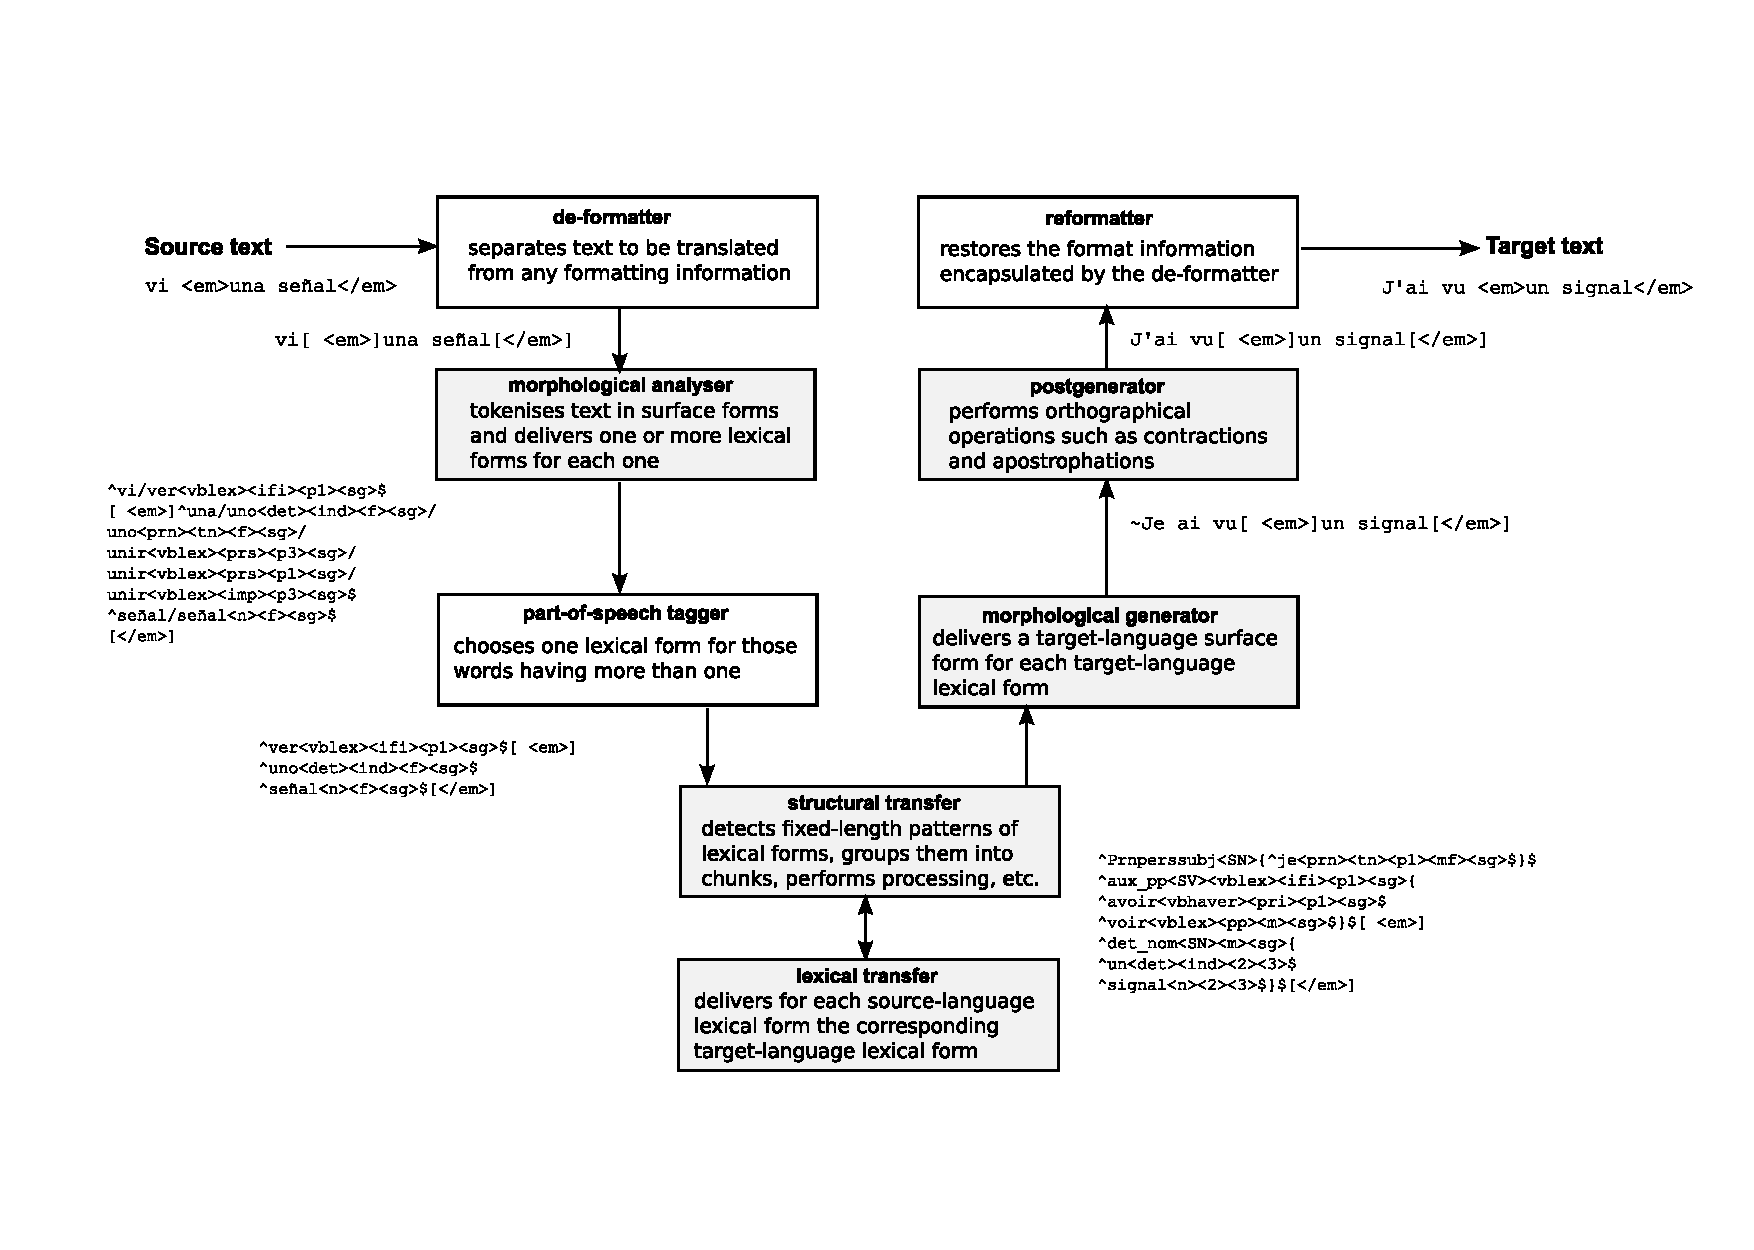
\includegraphics[width=1.2\textwidth]{apertium-general-architecture}}
    \tiny{(stock photage)}
    \label{fig:general-architecture}
  \end{figure}
\end{frame}


\subsection{\smenob{} pipeline}
\begin{frame}\frametitle{\smenob{} pipeline}
    \begin{figure}
    \begin{center}
      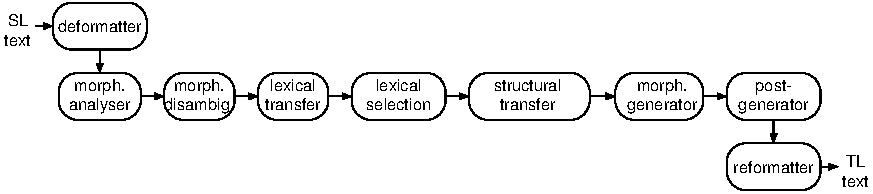
\includegraphics[width=1.0\textwidth]{../architecture}
    \end{center}
    \label{fig:modules}
  \end{figure}

    \vskip -0.1\textheight
  \begin{itemize}
  \item Analysis with HFST,
  \item lexical transfer and generation with lttoolbox
  \end{itemize}
  \begin{itemize}
  \item Disambiguation and lexical selection with Constraint
    Grammar
  \end{itemize}
  \begin{itemize}
  \item Four stage structural transfer
  \end{itemize}
\end{frame}

\subsection{HFST}
\begin{frame}\frametitle{Helsinki Finite State Tools}
  \begin{center}
    ``No, it isn't impossible to compile''
  \end{center}
  \begin{itemize}
  \item Drop-in replacement for proprietary-but-formerly-ubiquitous
    Xerox Finite State Tools
    \begin{itemize}
    \item lots of dictionaries now usable with FOSS tools
    \item loads quicker than Xerox tools :)
    \end{itemize}
  \end{itemize}

  \begin{itemize}
  \item More expressive power than lttoolbox, e.g. \textbf{flag
      diacritics}:
    \begin{itemize}
    \item in prefix paradigm: see a certain prefix, set a variable
    \item ... analyse some more of the word ...
    \item in suffix paradigm: only allow certain suffix if variable set
    \end{itemize}
  \item ... but slower          % nob is 21x faster than sme, but need comparable morphologies to test with
  \end{itemize}
\end{frame}

\section{Resources and development}
\begin{frame}
  \frametitle{Resources}
  \begin{itemize}
  \item \smenob{} translational dictionary, slightly machine-readable,
    9,900 lemmas
    \begin{itemize}
    \item Automatically converted
    \item ... manually excluding some
      ``explanatory'' entries, e.g. \textit{madda} $\rightarrow$
      \textit{branching part of deer's antlers}
    \item Many entries (semi-)manually entered
      \begin{itemize}
      \item now over 20,000, excluding proper nouns
      \end{itemize}

    \end{itemize}
  \end{itemize}
  \begin{itemize}
  \item \sme{} HFST analyser and CG disambiguator made by Giellatekno group
    at University of Tromsø
    \begin{itemize}
    \item Automatically converted, continually integrated
    \end{itemize}
  \end{itemize}
  \begin{itemize}
  \item \nob{} generator from \texttt{apertium-nn-nb}
    \begin{itemize}
    \item More or less unchanged
    \end{itemize}
  \end{itemize}
\end{frame}

\subsection{Analysis and derivations}
\begin{frame}\frametitle{Caring for your analyser: Trimming and pruning}
  \begin{itemize}
  \item Python script trims the analyser down to the translational
    lexicon, so we don't get ``half-translated'' words
    \begin{itemize}
    \item For each lemma + main-PoS in the analyser source files, look
      it up in the translational dictionary FST
    \item Only keep \sme{} analyser entries that have a corresponding
      entry in the translational dictionary
    \end{itemize}
  \end{itemize}
  \begin{itemize}
  \item \textbf{Two-level rules} prune out derivations that we don't
    yet know how to translate (well), giving priority to lexicalised
    words
  \end{itemize}
  \begin{itemize}
  \item Changes at Giellatekno continually merged in with minimal
    human effort
  \item Any additions added ``upstream''
  \end{itemize}
\end{frame}

\subsection{CG}
\begin{frame}\frametitle{Converting the disambiguator CG}
  \begin{itemize}
  \item Simple script to convert some tags
  \item Minor additions to e.g. favour full root analyses over
    derivations/compounds, fix disambiguation problems first noticed
    due to MT, added upstream
  \item Again, changes at Giellatekno continually merged in with
    minimal human effort
  \end{itemize}
\end{frame}

\begin{frame}\frametitle{Lexical selection}
  \begin{itemize}
  \item Rules created from scratch
  \item Tag and word sets copied from disambiguator
  \item Semantic sets from disambiguator useful here. E.g. the verb
    \textit{bivdit} translates into:
    \begin{itemize}
    \item \textit{spørre} (ask a question) if there's a
      question-particle to the right; else
    \item \textit{fiske} (fish) if there's a word from the \textsc{fish}
      semantic set in the sentence; else
    \item \textit{jakte} (hunt) if there's a word from the
      \textsc{nature-place}/\textsc{hunt-animal}/\textsc{bird} sets or
      the verb itself has the Actor derivation; else
    \item \textit{be} (ask something of someone)
    \end{itemize}
  \end{itemize}
\end{frame}

\subsection{Transfer}
\begin{frame}\frametitle{Tag transfer}
  \begin{itemize}
  \item \sme{} analyser created outside Apertium project, very
    different tagset
  \item CG as well, and it expects the analyser tagset
  \item So we ``translate'' tags during translation, using lots of
    paradigms (=continuation lexicons) in the translational dictionary
  \item Main source of bugs and frustration; difficult to foresee the
    possible tag and derivation combinations
  \end{itemize}
\end{frame}

\begin{frame}\frametitle{Structural transfer -- grammar!}
\begin{enumerate}
\item Chunking, 63 rules
  \begin{itemize}
    \item NP chunking
    \item NP with adverbial case $\rightarrow$ \textsc{prep} + NP
    \item causative, reflexive verb $\rightarrow$ `let' + \textsc{v} + \textsc{pron.refl}
  \end{itemize}

\item Interchunk 1, 26 rules
  \begin{itemize}
  \item simple anaphora resolution
  \item merge coordinated NP chunks
  \item NP \textsc{postp} $\rightarrow$ \textsc{prep} NP
  \end{itemize}

\item Interchunk 2, 39 rules
  \begin{itemize}
  \item major word order changes
  \item insert dropped pronouns
  \item insert adverbs to indicate verb modality
  \item correct NP definiteness using verb information
  \end{itemize}

\item Postchunk, 29 rules
  \begin{itemize}
  \item insert determiners, infinitive marker
  \item tag cleanup
  \end{itemize}
\end{enumerate}
\end{frame}

\begin{frame}\frametitle{Derivations}
  \begin{itemize}
  \item Derivations involve a lot of guessing and sometimes odd
    translations, especially when changing PoS
  \item We do \textit{not} invent suffixes:
    \begin{itemize}
    \item `clear' as a noun, is it: `clearhood'? `clearness'?
      `clearment'? `clearship'? `clearerty'? (`clarity')
    \item `unemployed' as a noun, is it: `unemployedhood'?
      `unemployedness'? `unemployity'? `unemployedship'?
      (`unemployment')
    \end{itemize}
  \item We pick from \textit{possible} forms, taking advantage of
    \nob{} PoS ambiguity:
    \begin{itemize}
    \item The \nob{} word \textit{bygger} is ambiguous between the
      present tense of `build' or the Actor noun `builder'; so we tag
      transfer \textsc{v.der.actor.n} $\rightarrow$ \textsc{v.pres}
    \end{itemize}
  \item Causative derivation: no PoS change, but insert auxiliary
  \end{itemize}
\end{frame}

\begin{frame}
  \frametitle{Derivations}
  \begin{itemize}
  \item Derivations lead to transfer complexity
    \begin{itemize}
    \item verbs in NP chunks and vice versa
    \item double derivations, words where the lemma has a
      ``hardcoded'' PoS change in the translational dictionary
    \end{itemize}
  \item Lexicalised entries, however, translate directly into the
    right lemma+PoS, no guessing, no added transfer complexity
  \item But lexicalising takes time, and derivations increase coverage
  \item We keep derivation types if they are high frequency and we
    find an acceptable way of translating them
  \item Assimilation priorities: preserve meaning, avoid untranslated
    words
  \end{itemize}
\end{frame}

\section{Evaluation}
\begin{frame}\frametitle{Evaluation}
  \begin{itemize}
  \item Coverage and ambiguity
  \item Word Error Rate (WER)
  \item ``Gisting'' questionnaire
  \end{itemize}
\end{frame}

\subsection{Coverage, WER}
\begin{frame}\frametitle{Coverage and ambiguity rate}
  \begin{center}
    \begin{table}
      \begin{tabular}{crrrrr}
        Corpus     & tokens   & coverage & ambig.      & coverage   & ambig.rate  \\
        &          &          & rate        & w/o deriv  & w/o deriv \\
        laws       &  51706   & 94.68\%  & 2.65        & 86.02\%    & 2.32 \\
        wiki       & 19942    & 77.52\%  & 2.36        & 74.56\%    & 2.19 \\
        news       & 1020250  & 94.72\%  & 2.59        & 90.96\%    & 2.34 \\
      \end{tabular}
      \caption{Na\"{i}ve coverage on several corpora.}
      \label{table:cov}

      (ambiguity rate reduced to about 1.04 by CG rules)
    \end{table}
  \end{center}
\end{frame}

\begin{frame}\frametitle{Word Error Rate}
  \begin{table}
    \begin{center}
      \begin{tabular}{ccrrr}
        Text       & tokens & Unknown & WER  \\
        children's & 415     & 5      & 45.96\% \\
        history    & 435     & 28     & 60.32\%  \\
      \end{tabular}
      \caption{Word error rate on two short texts.}
      \label{table:wer}
    \end{center}
  \end{table}
\end{frame}

\subsection{Gisting eval}
\begin{frame}\frametitle{Gisting eval: test 1, multiple paraphrase choice}
  \ex.
  \texttt{Original:} \textit{Muhto eat diehtán maid mii čáliimet} \textcolor{blue}{(`But we didn't know what we wrote')}\\
  \texttt{Translated:} \textit{Men vi visst ikke også skrev vi} \textcolor{blue}{(`But we didn't known also wrote we')}\\
  \texttt{Pick the right alternative:}\\
  \a. \textit{Vi visste hva vi skrev} \textcolor{blue}{(`We knew what we wrote')}\\
  \b. \textit{Vi visste ikke hva vi skrev} \textcolor{blue}{(`We didn't know what we wrote')}\\
  \c. \textit{Vi visste ikke hva de skrev} \textcolor{blue}{(`We didn't know what they wrote')}

  % Always empty line after \ex.!
\end{frame}

\begin{frame}\frametitle{Gisting eval: test 2, open question}
  \ex.
  \small
  \texttt{Original:} \textit{Goappaš riikkain lea nammaduvvon hálddahuslaš gulahallanolmmoš} \textcolor{blue}{(`There is appointed an administrative contact from both countries')}\\
  \texttt{Translated:} \textit{Goappaš på rikene er det oppnevnt administrativt forstående hverandre seg mennesket} \textcolor{blue}{(`Goappaš on the countries there is appointed an administrative understanding eachother self person')}\\
  \texttt{Answer the question:} \textit{Hvor kommer kontaktpersonene fra?} \textcolor{blue}{(`Where do the contact persons come from?')}\\~\\
  \_\_\_\_\_\_\_\_\_\_\_\_\_\_\_\_\_\_\_\_\_\_\_\_\_\_\_\_\_\_\_\_\_\_\_\_\_\_\_\_

  % Always empty line after \ex.!
\end{frame}

\begin{frame}\frametitle{Gisting eval: test 3, multiple word choice}
  \ex.
  {\footnotesize
    \texttt{Original:} \textit{Lahttu, gean stáhta lea nammadan, lea lávdegotti jođiheaddji}\\
    \textcolor{blue}{(`The member, who the Government has instituted, is the committee's leader')}\\
    \texttt{Translated:} \textit{Medlemmet, som staten har oppnevnt, det er komiteens leder}\\
    \textcolor{blue}{(`The member, who the Government has instituted, that is the leader of the committee')}\\
    \texttt{Pick the right alternative:}
    \textit{Medlemmet oppnevnt av}\\
    \textsc{$\square$grunnen $\square$staten $\square$kommunen $\square$lederen $\square$komiteen $\square$haustaren $\square$(ingen som passer)}\\
    \textit{er leder for}\\
    \textsc{ $\square$sjøen $\square$komiteen $\square$vurderingen $\square$dommen $\square$gangen $\square$utgangen $\square$(ingen som passer)}\\
    \textcolor{blue}{(`The member instituted by the\\
    \textsc{$\square$grounds $\square$Government $\square$County $\square$leader $\square$committee $\square$harvester $\square$(none of the above)}\\
    is the leader of the\\
    \textsc{$\square$sea $\square$committee $\square$assessment $\square$verdict $\square$time $\square$closing $\square$(none of the above)}')}
  }

  % Always empty line after \ex.!
\end{frame}

\begin{frame}\frametitle{Results}
  \begin{table}[htdp]
    \caption{Results of gisting evaluation, 3 different tests}
    \begin{center}
      \begin{tabular}{lccc}
        Type & Paraphrases & Open question & Generated \\
        Result & 77 \% & 41 \% & 75 \% \\
        N test subjects & 10 & 14  & 10  \\
      \end{tabular}
    \end{center}
    \label{eval}
  \end{table}

  % \begin{itemize}
  % \item
  % \end{itemize}
\end{frame}

\section{Conclusion}
\begin{frame}\frametitle{Future work}
  \begin{itemize}
  \item More structural transfer rules, we don't catch all major
    constructions
  \item Automatically create lexical selection rules with
    \tool{apertium-lex-tools}
  \item Better disambiguation: improve rules, perhaps train HMM
  \item More entries for the translational dictionary
  \end{itemize}
\end{frame}

\begin{frame}\frametitle{Licences}
  This presentation may be distributed under the terms of the
  GNU GPL, GNU FDL and CC-BY-SA licences.
  \begin{itemize}
  \item GNU GPL v. 3.0 \\
    \href{http://www.gnu.org/licenses/gpl.html}{http://www.gnu.org/licenses/gpl.html}
  \item GNU FDL v. 1.2 \\
    \href{http://www.gnu.org/licenses/gfdl.html}{http://www.gnu.org/licenses/gfdl.html}
  \item CC-BY-SA v. 3.0 \\
    \href{http://creativecommons.org/licenses/by-sa/3.0/}{http://creativecommons.org/licenses/by-sa/3.0/}
  \end{itemize}
\end{frame}


% \begin{frame}[fragile]\frametitle{code example}
%   \begin{verbatim}
%   verbatim text needs to be in fragile frames
%   \end{verbatim}
% \end{frame}



\end{document}
